\documentclass[12pt]{article}
\usepackage{graphicx}
\usepackage{amsmath}   % for having text in math mode

%Following 2 lines were added to remove the blank page at the beginning
\usepackage{atbegshi}% http://ctan.org/pkg/atbegshi
\AtBeginDocument{\AtBeginShipoutNext{\AtBeginShipoutDiscard}}
%

\begin{document}

\begin{center}
\title{\textbf{Area of a Traingle}}
\date{\vspace{-5ex}} %Not to print date automatically
\maketitle
\end{center}

\setcounter{page}{1}



\section{10$^{th}$ Maths - Chapter 7}

All problems are from Exercise 7.3

\begin{enumerate}
\item Find the area of the triangle whose vertices are :
\begin{enumerate}
\item $(2, 3), (–1, 0), (2, – 4)$
\item $(–5, –1), (3, –5), (5, 2)$ 
\end{enumerate}

\item In each of the following, find the value of '$k$', for which the points are collinear.
\begin{enumerate}
\item $(7, –2), (5, 1), (3, k)$
\item $(8, 1), (k, – 4), (2, –5)$
\end{enumerate}

\item Find the area of the triangle formed by joining the mid-points of the sides of the triangle whose vertices are $(0, –1), (2, 1) \text{ and } (0, 3)$. Find the ratio of this area to the area of the given triangle.

\item Find the area of the quadrilateral whose vertices, taken in order, are $(– 4, – 2), (– 3, – 5), (3, – 2) \text{ and } (2, 3)$.

\item You have studied in Class IX, (Chapter 9, Example 3), that a median of a triangle divides it into two triangles of equal areas. Verify this result for $\triangle ABC$ whose vertices are $\vec{A}(4, -6), \vec{B}(3, 2), \text{ and } \vec{C}(5, 2)$. 

\end{enumerate}

\section{12$^{th}$ Maths - Chapter 8}
\begin{enumerate}
\item Using integration find the area of region bounded by the triangle whose
	vertices are $(1, 0), (2, 2) \text{ and } (3, 1)$ as shown in Figure \ref{fig:Fig1}. (Ref : Example 9)

\begin{figure}[!h]
	\begin{center}
	    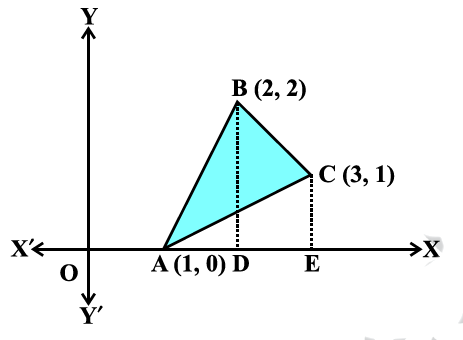
\includegraphics[width=\columnwidth]{./fig1}
	\end{center}
\caption{}
\label{fig:Fig1}
\end{figure}

\item Using integration find the area of region bounded by the triangle whose vertices
	are $(– 1, 0), (1, 3) \text{ and } (3, 2)$. (Ref : Problem 4 in Ex 8.2)

\item Using the method of integration find the area of the $\triangle$ ABC, coordinates of whose vertices are $\vec{A}(2, 0), \vec{B}(4, 5), \text{ and } \vec{C}(6, 3)$. (Ref: Problem 13 in Misc Exercise on Chapter 8)

\end{enumerate}


\end{document}
